\subsection{Faithful Generation and Why Models Make Semantic Errors}

We now formally define faithfulness as it relates to \meaningrepresentation~to
text generation.
Let $\GEN : \mrspace \rightarrow \outSpace$ be an arbitrary mapping from 
\meaningrepresentations~to utterances. We say that a mapping $\GEN$ is 
\faithful~if we have that \[\denotes{\GEN(\mr)} = \mr \quad \forall \mr: \mr \in \mrspace.\] In words,
$\GEN$ is faithful if the propositional content of $\mr$ (i.e., the semantics
of the \attributevalue~pairs in $\mr$) is correctly expressed by the 
generated utterance $\predutttoks = \GEN(\mr)$ for any well-formed \meaningrepresentation~$\mr$. 

If $\GEN$ is implemented with templates like in \cite{puzikov2018},
it is possible to design a faithful mapping. However, it is possible that 
faithfuless and naturalness are in tension, as the method of \cite{puzikov2018}
did not performance highly on human judgements of naturalness.

It is well known that implementing $\GEN$ with a neural model $\gen$ and 
an inference procedure like beam search are not sufficient to obtain a faithful
model.  The bias inherent to beam search means that 
low-perplexity utterances are 
more likely to be generated rather than semantically correct utterances \citep{serban2016}. 
 As mentioned in \autoref{sec:nlginference},  a common approach to make $\gen$ more faithful is to perform overgeneration 
 with
reranking \citep{dusek2016,juraska2018,dusek2019,dusek2020}. 
The $\nbest$-best list of utterances $\mathcal{H}_{complete} = \left\{\utttoks^{(1)},\ldots,
\utttoks^{(\nbest)}\right\}$ is produced using beam search with $\gen\left(\cdot|\ls(\mr)\right).$
Then 
a discriminative \meaningrepresentation~parser, $\dmodel(\cdot|\cdot) : \mrspace \times \outSpace \rightarrow (0,1)$, is used to rerank $\mathcal{H}_{complete}$ such
that the final output utterance is \[
\predutttoks = \argmax_{\utttoks \in \mathcal{H}_{complete}} \dmodel\left(\mr\vert\utttoks\right). \]
In this setting the inference procedure selects the 
utterance that 
that most likey denotes the input $\mr$ under $\dmodel$. While this reduces the risk of
generating an incorrect utterance with respect to $\mr$, it can still fail
when either $\dmodel$ is not accurate or when $\mathcal{H}_{complete}$ does not contain
a completely correct utterance.

The critical issue here is that the final beam search hypothesis set may
not contain any completely semantically correct utterances.
This in part happens because neural models on natural language data\footnote{Here we are referring to both \sequencetosequence~models but also 
sequence classification \citep{kim2014convolutional,mccoy2019} 
and sequence-pair classification \citep{snli}. }  do not 
na{\"i}vely exhibit the quality of systematicity \citep{fodor1988,phillips1998,marcus2003,lake18,mccoy2019,gardner2020}. A model displays systematicity if
 the capability of the model to  perform a task implies that it can perform
other structurally related tasks successfully.
%a task correctly does not imply that a ne
On natural language data, a model with systematicity should be able to exploit the algebraic and compositional 
nature of natural language to make correct inferences. \citet{lake18} give the example of a human
speaker that understands the concept of ``twice'' or ``again,'' who, upon
learning a novel verb, ``to dax,'' immediately understands the meaning 
of ``daxed twice'' or ''to dax again'' even though they have never seen 
examples of these compositions before. Empirically, they demonstrate that a
\recurrentneuralnetwork~based \meaningrepresentation-to-text model ({\color{red} check direction}) does not posses this ability and frequently fails to 
generalize to novel compostions even where the individual constituents of 
the compositions are well represented in the training data.

In our present case, this lack of systematicity manifests itself as a failure
to realize individual \attributevalues~that are well represented in the 
training data when those \attributevalues~occur in novel combinations in a 
 \meaningrepresentation~at test time. We use as a case-study, the \attributevalue~``near=Burger King.'' which in our restaurant domain dataset, the E2E Challenge dataset \citep{dusek2018}, denotes that a restaurant $x$ is near
Burger King. 


The \attributevalue~\AV{near}{Burger King} appears frequently in the training
data in longer \meaningrepresentation/utterance pairs. In fact \AV{near}{Burger King} is positively associated with \meaningrepresentations where seven or eight \attributes~are specified (there are eight total unique attributes on this
dataset). See \autoref{fig:bkpmi} where we plot the point-wise mutual information
(PMI) \citep{church1990} of the occurrence of the \AV{near}{Burger King} and the occurrence of a \meaningrepresentation~of a particular size on the training set, where the size of a \meaningrepresentation~$\setsize{\mr}$ is the number of \attributevalue~pairs in $\mr$.
The PMI is computed as 
\[\pmi(\AV{near}{Burger King},  \setsize{\mr} = k) = \log \frac{p(\AV{near}{Burger King}, \setsize{\mr} = k)}{p( \AV{near}{Burger King}  ) p(\setsize{\mr} = k)}     \quad \forall k : k \in \{3,\ldots,8\},\]
with \begin{align*}
    p(\AV{near}{Burger King}) &= \frac{\sum_{(\mr,\utttoks) \in \corpus}\mathds{1}\left\{ \AV{near}{Burger King} \in \mr \right\}}{\setsize{\corpus}} \\
    p(\setsize{\mr}=k) &= \frac{\sum_{(\mr,\utttoks) \in \corpus}\mathds{1}\left\{ \setsize{\mr} = k \right\}}{\setsize{\corpus}} \\
    p(\AV{near}{Burger King},\setsize{\mr}=k) &= \frac{\sum_{(\mr,\utttoks) \in \corpus}\mathds{1}\left\{\AV{near}{Burger King} \in \mr \wedge \setsize{\mr} = k \right\}}{\setsize{\corpus}}.
\end{align*}
From \autoref{fig:bkpmi} we can see that \AV{near}{Burger King}~is negatively
associated with smaller \meaningrepresentations, suggesting a neural
model will struggle to generate utterances for it in the smaller \meaningrepresentation~regime.

\begin{figure}[t]
\centering
    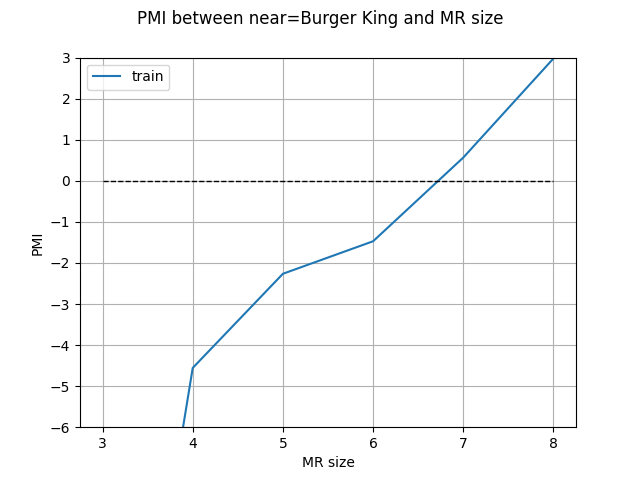
\includegraphics[scale=0.5]{nlg/nearbk.png}
\caption{PMI between \AV{near}{Burger King}~and \meaningrepresentation~size
on the E2E Challenge dataset. 0 on the $y$-axis indicates the two variables are independent.}
\label{fig:bkpmi}
\end{figure}


To demonstrate this, we trained a uni-directional GRU generation model on the training corpus
and then tried to generate an utterance for the following \meaningrepresentation,
\begin{center}
    \MR{\textsc{Inform}}
        {\AV{name}{Alimentum}}  
        {\AV{near}{Burger King}}
        {\AV{area}{city centre}}
        {\AV{family\_friendly}{no}}\end{center}
using beam search. Notice that in this case $\setsize{\mr}=4$,
indicating that the occurrence of \AV{near}{Burger King} is a 
relatively novel situtation given
 the training set.
We generated some beam search canditates we we show below, {\color{red}\uline{underlining in red}} the phrases that
are not semantically correct given the \meaningrepresentation,

\begin{enumerate}
\item Alimentum is located in the city centre {\color{red}\uline{near the Express by Holiday Inn.}} It is not family-friendly.     
\item Alimentum is located in the city centre {\color{red}\uline{near the Yippee Noodle Bar.}} It is not family-friendly.
\item Alimentum is located in the city centre {\color{red}\uline{near the Raja Indian Cuisine.}} It is not family-friendly.
\item Alimentum is not family-friendly. It is located in the city centre {\color{red}\uline{near the Yippee Noodle Bar.}}
\item The Alimentum is located in the city centre {\color{red}\uline{near the Express by Holiday Inn.}} It is not family-friendly.
%Alimentum is not family-friendly. It is located in the city centre near the Raja Indian Cuisine.\\\vspace{-1em}\\
%Alimentum is located in the city centre near the Clare Hall. It is not family-friendly.\\\vspace{-1em}\\
%Alimentum is located in the city centre near the crowne plaza hotel. It is not family-friendly.\\\vspace{-1em}\\
%Alimentum is not family-friendly. It is located in the city centre near the express by holiday inn.\\\vspace{-1em}\\
%The Alimentum is located in the city centre near the Yippee Noodle Bar. It is not family-friendly.\\\vspace{-1em}\\
%Alimentum is not family-friendly. It is located in the city centre near the Clare Hall.\\\vspace{-1em}\\
%The Alimentum is located in the city centre near the Raja Indian Cuisine. It is not family-friendly.\\\vspace{-1em}\\
%In the city centre near the express by holiday inn is Alimentum. It is not family-friendly.\\\vspace{-1em}\\
%Alimentum is located in the city centre near the city centre. It is not family-friendly.\\\vspace{-1em}\\
%Alimentum is located in the city centre near the rice boat. It is not family-friendly.\\\vspace{-1em}\\
%The Alimentum is not family-friendly. It is located in the city centre near the Yippee Noodle Bar.\\\vspace{-1em}\\
%Alimentum is located in the city centre near the rainbow vegetarian café. It is not family-friendly.\\\vspace{-1em}\\
%In the city centre near the Yippee Noodle Bar is the Alimentum. It is not family-friendly.\\\vspace{-1em}\\
%In the city centre near the Yippee Noodle Bar is Alimentum. It is not family-friendly.\\\vspace{-1em}\\
%
\end{enumerate}
Right away we are confronted by their homogeneity; utterances 1,2,3 and 5
have the same syntactic structure, varying only in the phrase \textit{near x}.
Utterances 1 and 5 differ only by a single word (the initial article \textit{The} in 5).  Most importantly, none of them correctly specify that the Alimentum 
is near Burger King. Even with a beam size of 128, the phrase \textit{Burger King} is never generated by the model!\footnote{A beam size of 128 would be impractial for most applications. Beam sizes are typically from 4-10 in most works.}


\begin{figure}[p]
\centering
    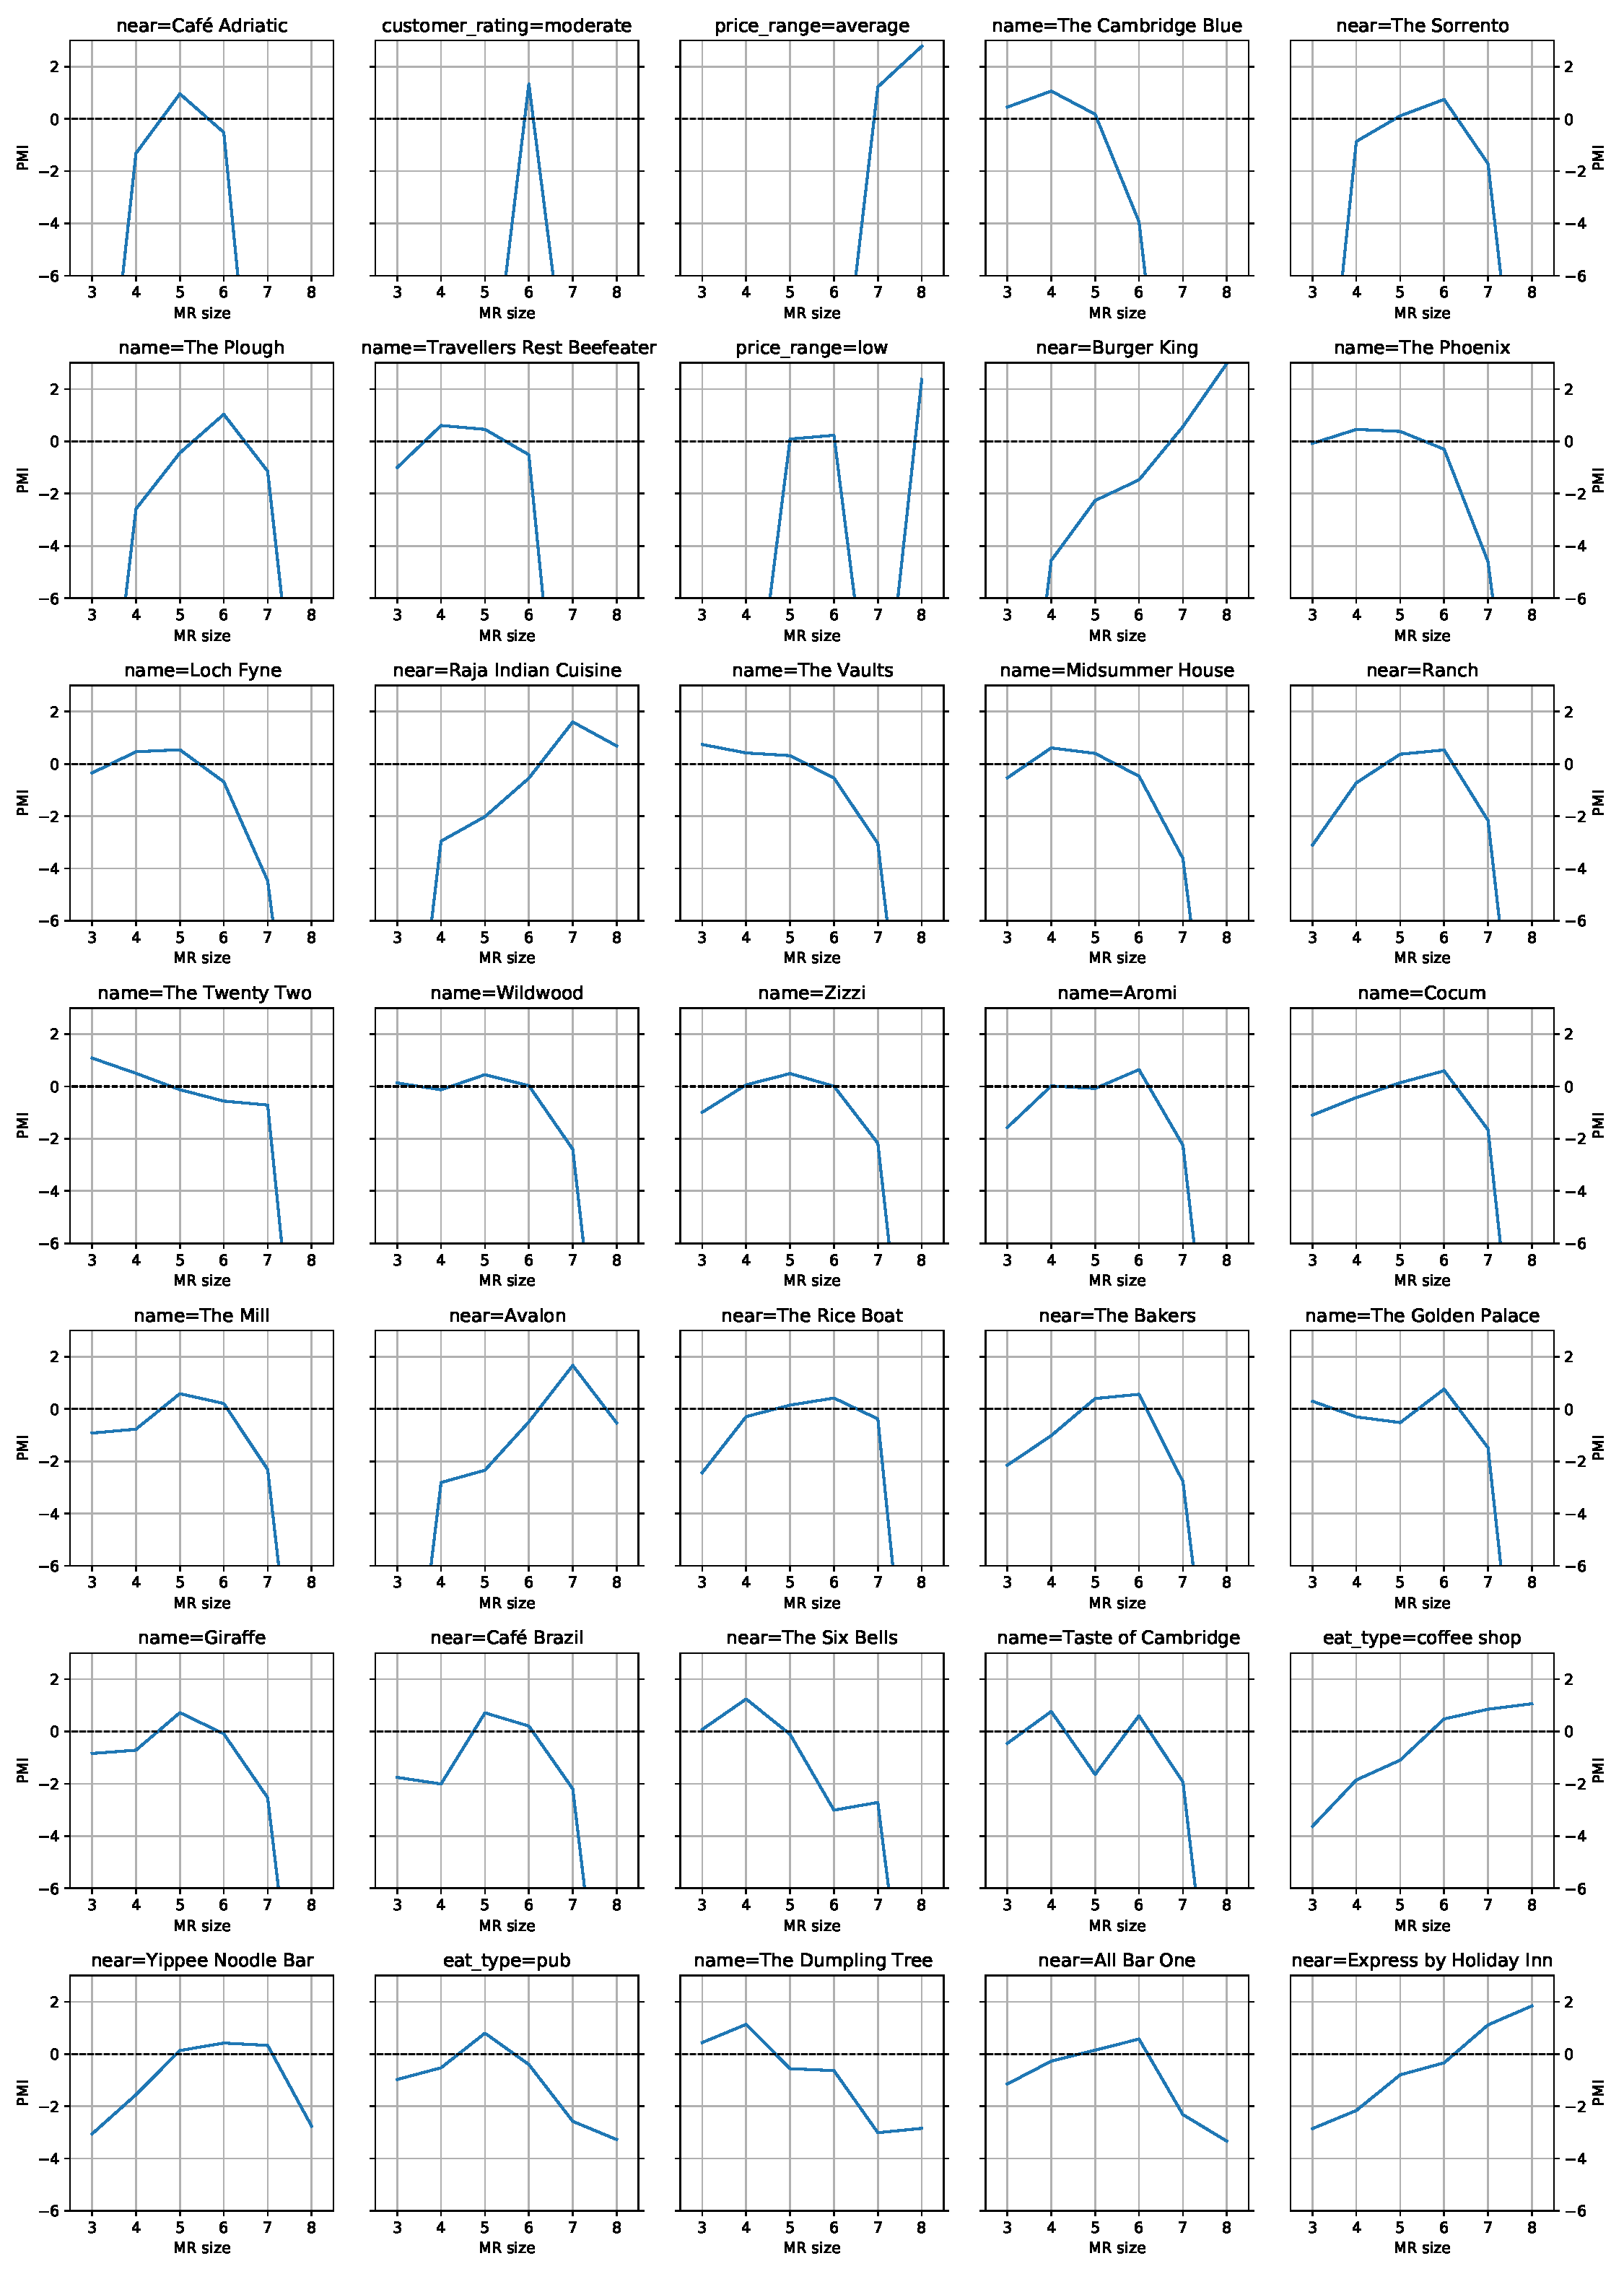
\includegraphics[width=0.9\textwidth]{nlg/trainpmis.pdf}
\caption{PMI between various \attributevalue s and \meaningrepresentation~size
on the E2E Challenge dataset. 0 on the $y$-axis indicates the two variables are independent.}
\label{fig:trainpmi}
\end{figure}


This is more frustrating because there are plenty of training examples where
even a coarse understanding of phrase structure would allow construction
of a correct utterance for this case.
For instance, we observe utterances containing \textit{near Burger King}
like this,
\begin{quotation}
\noindent \textit{The Eagle is a low rated coffee shop \textbf{near Burger King}
and the riverside that is family friendly and is less than £20
for Japanese food.}
\end{quotation}
while also seeing
\begin{quotation}
\noindent \textit{Alimentum is located in the city centre \textbf{near Yippee Noodle Bar}. \textellipsis}
% It serves expensive Italian food. It has an average customer rating.
\end{quotation}
where a correct utterance could be created by substituting ``Burger King''
in the latter instance, e.g., 
\begin{quotation}
\noindent \textit{Alimentum is located in the city centre \textbf{near Burge King}.}
% It serves expensive Italian food. It has an average customer rating.
\end{quotation}

Unfortunately, the GRU model does not learn to substitute the correct 
prepositional phrase. Given that correct examples seem constructable from
constituent phrases, it suggests that a data-augmentation approach
might help to generate additional training examples that do not possess 
some of the spurious correlations between \attributevalue s and input size.

Indeed, the compositional data-augmentation scheme proposed by \citet{andreas2020} demonstrates  improved model systematicity.
Unfortunately, a rule based system of recombination risks creating 
disfluencies in the utterances that could potentially reduce the fluency
of the learned model. Additionally, the number of spurious
associations in the dataset are numerous; see \autoref{fig:trainpmi} for 35 of the
total {\color{red}???} \attributevalue~pairs for the E2E dataset. They all have some 
spurious association with \meaningrepresentation~size. And we haven't even
explored other associations that might exist (e.g. between two \attributevalue~pairs). In the following subsections, we explore what an ideal
 data-augmentation policy might look like and then give a practical 
implementation of it.



%?This suggests that a data-augmentation strategy,
%?perhaps we can perform some recombination
%?of various trainging phrases and fragments, e.g. construct the example
%?This kind of data-augmentation has been helpful in making 
%?models behave more systematically \citep{thethinsg.}. 


%\clearpage

